
\chapter{Literature Review}
\label{chap:literature_review}

\section{Weather Nowcasting}
\label{sec:nowcasting}


When asked to predict future rainfall, meteorologists often get it wrong. At first glance, forecasting rainfall should be manageable as it is one of the main focuses of weather predictions, but the opposite turns out to be the case. Rain is tough to forecast on a small scale.

Rainfall forms in two main ways. The first one happens when two fronts of different temperatures meet. Because of that, it is called frontal rain. The warmer air mass is lifted above, the colder as it is less dense. It then cools at a higher altitude, which causes the water trapped in the previously warmer air to condense due to a drop in the temperature. Meteorologists can predict this type of rainfall by studying these air masses using available weather instruments. Frontal rain often lasts longer and amounts to 40 percent of all rainfall.

The other 60 percent comes from a process known as convection. This type of rain happens when the ground warmed by the sun transfers heat to the nearby air. Warming can cause the air to rise to the higher layers of the atmosphere, where the water vapor condenses. Convective rainfall sounds very similar to frontal rain. Predicting precipitation accurately can be challenging due to several factors. These include determining the ground's temperature, whether the heat is enough to make the air rise, and how long the air will stay above the warm ground to absorb the heat. Knowing the amount of water vapor in the air mass is also crucial. The areas this type of rain covers are minor and likely undetectable by methods used for frontal rain predictions. Convective rain is also shorter and, therefore, harder to predict.

Weather nowcasting aims to address predictions in this shorter horizon. Keith Browning originally defined it as \textit{``the description of the current state of the weather in detail and the prediction of changes that can be expected on a timescale of a few hours''}\cite{browningnowcating}. Later, the \gls{WMO} defined \textit{nowcasting} as forecasting with local detail, by any method, over a period from the present to 6 hours ahead, including a detailed description of the current weather.

\subsection{Radars}
\label{subsec:radars}

Nowcasting is highly dependent on observational data. While surface and upper-air observations are essential, only remote sensing systems can adequately provide high-resolution spatial coverage. A weather radar is the most crucial instrument for nowcasting, particularly for severe local storms associated with thunder, lightning, heavy rain, hail, strong winds, and sudden temperature changes.

Radar has an advantage over all other observing systems in weather forcasting because it directly observes precipitation particles in three dimensions over a large area with an update rate of a few minutes. At radar ranges of less than 60 kilometers, the resolution of the precipitation is better than 1 kilometer squared. Radar makes it possible to estimate rainfall rates and amounts, observe the 3D structure of a storm, which has proven useful in estimating storm severity, and obtain the movement of storms, which is central to nowcasting. With the addition of Doppler capability\footnote{Doppler shift of the radar waves allows the radar to determine the speed and direction (only toward or away from the radar) of precipitation particles.}, it is possible to estimate the wind direction and speed. The further addition of dual-polarization\footnote{Transmitting and receiving two differently polarized waveforms.} enables differentiation of the precipitation particle type, such as rain, snow, or hail, and to identify non-precipitation echoes, such as insects and ground clutter. Dual polarization is particularly useful for data quality control. \cite{nowcastingguidlines}

The radar collects the measurements in reflectivity, a measure of the power returned to the radar, from atmospheric targets, such as raindrops, snow\-flakes, or hailstones. The radar reflectivity is measured in dBZ and is represented on a logarithmic scale in decibels (dB) to accommodate the observations in a wide range of signal strengths. The unit dBZ expresses radar reflectivity relative to a reference value (Z), which is the radar reflectivity of a 1 mm diameter droplet of water at a standard distance from the radar. The higher the radar reflectivity, the more intense the precipitation is likely to be.

Radar attributes, such as radar wavelength, Doppler capabilities, dual-polarization, sensitivity, and scanning capabilities, affect the radar's abilities. The primary one is the radar wavelength. There are three wavelengths: S-band ($~$10 cm), C-band ($~$5 cm), and X-band ($~$3 cm). For example, if the primary use of the radar is for estimating heavy rainfall over large regions and to warn of high-wind events from thunderstorms, then an S-band, Doppler, dual-polarization radar is the most suitable. However, if the primary use of the radar is for nowcasting snow, then C-band or even X-band may be suitable. \cite{nowcastingguidlines}

\section{Convolutional Neural Networks}
\label{sub:cnn}

\glspl{NN} are computational models inspired by biological neural networks. Their goal is to minimize errors between outputs and given target values computed by loss function, e.g., \gls{MSE}. The function is minimized by adjusting the weights inside the network based on these errors using error backpropagation and gradient descent algorithm\footnote{I will not go into the inner workings of this algorithm, as it is not the main focus of this thesis. I assume a basic understanding of forward and backward passes from the reader in feed-forward \glspl{NN}. See paper \cite{backpropagation} in which was the backpropagation first proposed.}. After a sufficient number of successive adjustments, \gls{NN} produces an output similar to the target output, and the training can be terminated based on specific criteria. \glspl{NN} can theoretically learn to represent and model any given continuous function, no matter how complex, as long as the network has an appropriate architecture and the function is well-defined within a particular domain \footnote{See paper \cite{universalapproximators}}.

\glspl{CNN} first appeared in the 90s, but their widespread use can be attributed to breakthroughs in the ImageNet image classification challenge \cite{cnn}. \glspl{CNN} have enormously impacted the world of image processing, making them a worthy candidate for predicting the weather phenomena captured in radar images. \glspl{CNN} leverage ideas, such as sparse interactions, parameter sharing, and equivariant representations, to improve machine learning systems. To understand the benefits convolutional \glspl{CNN} bring, I need to introduce a mathematical operation that makes \gls{CNN} a \gls{CNN}.

\subsection{Convolution}
\label{subsec:convolution}

Under the hood \glspl{CNN} use, as the name implies, an operation called convolution. Bread and butter of \glspl{NN} are affine transformations. Vector of inputs is received, then multiplied by some transformation matrix\footnote{A bias vector is added before passing the result to non-linear function}. These operations can be applied to various input types, such as images or sounds. Every input can be represented as a multi-dimensional array, which can then be flattened to apply the transformation. There often are dimensions along which ordering of the data matters\footnote{Width and height of images or time axis in sound}. Similarly, the data often has something we can call ``channel axis'', which represents different views of the data \footnote{Different color channels in images or audio channels in sound}. Flattening the data does not consider these relationships, which may be important in solving tasks like computer vision and speech recognition. \cite[pg. 6-8]{convolutionguide}

Discrete convolution is the answer to this concern. An excellent way to imagine the convolution operation is through a window called the kernel, sliding across the input. The input values are multiplied by the corresponding value in the overlapping window and summed up to obtain the convolution output in the window's current location. The window is then moved to the next position. Output for all valid kernel positions\footnote{Position of a kernel on top of input is valid when an input value exists for every kernel value.} is called output feature map. This whole procedure can be repeated with many more kernels to form as many output feature maps as desired. In figure \ref{fig:convolution_slide}, we see an example of convolution with 4×4 input and 3×3 kernel. From now on, I will focus on 2D convolution, in which the input and the kernel are two-dimensional.

\begin{figure}[ht]
    \centering
    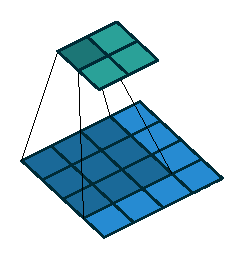
\includegraphics[width=0.24\textwidth]{images/no_padding_no_strides_00.pdf}
    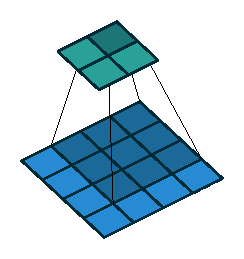
\includegraphics[width=0.24\textwidth]{images/no_padding_no_strides_01.pdf}
    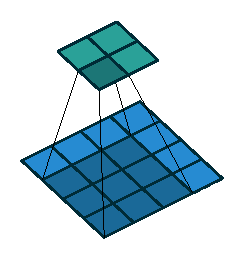
\includegraphics[width=0.24\textwidth]{images/no_padding_no_strides_02.pdf}
    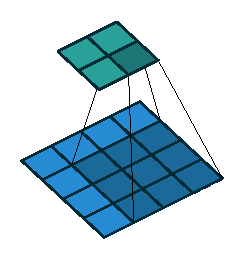
\includegraphics[width=0.24\textwidth]{images/no_padding_no_strides_03.pdf}
    \caption[2D convolution with 4×4 and 3×3 kernel]{\label{fig:convolution_slide}
    Convolving a 3×3 kernel over a 4×4 input. \cite{convolutionguide}}
\end{figure}

There can be several feature maps in the input, e.g., representing different image color channels. In that case, the kernel can have multiple dimensions. Using a multi-dimensional kernel is equivalent, to creating the output feature map, by using multiple kernels and summing the resulting unique feature maps element by element. The usage of a collection of kernels to both create multiple output feature maps and convolve over input with multiple channels is illustrated in figure \ref{fig:convolution_kernel_collection}.

\begin{figure}[ht]
    \centering
    \begin{tikzpicture}[scale=.35,every node/.style={minimum size=1cm}, on grid]
        \begin{scope}[xshift=0cm,yshift=4cm]
            \begin{scope}[xshift=0cm,yshift=0cm]
                \draw[draw=base03,fill=violet,thick]
                (0,0) grid (5,5) rectangle (0,0);
            \end{scope}
            \begin{scope}[xshift=0.5cm,yshift=0.5cm]
                \draw[draw=base03,fill=blue,thick]
                (0,0) grid (5,5) rectangle (0,0);
            \end{scope}
        \end{scope}
        \foreach \y in {0,5,10} {%
            \begin{scope}[yshift=\y cm,xshift=10cm]
                \begin{scope}[xshift=0cm,yshift=0cm]
                    \draw[draw=base03,fill=violet,thick]
                    (0,0) grid (3,3) rectangle (0,0);
                \end{scope}
                \begin{scope}[xshift=0.5cm,yshift=0.5cm]
                    \draw[draw=base03,fill=blue,thick]
                    (0,0) grid (3,3) rectangle (0,0);
                \end{scope}
            \end{scope}
            \begin{scope}[yshift=\y cm,xshift=20cm]
                \begin{scope}[xshift=0.5cm]
                    \draw[draw=base03,fill=cyan,thick]
                    (0,0) grid (3,3) rectangle (0,0);
                \end{scope}
            \end{scope}
        }
        \begin{scope}[xshift=30cm,yshift=4.75cm]
            \foreach \s in {0.0,0.5,1.0} {%
            \begin{scope}[xshift=\s cm,yshift=\s cm]
                \draw[draw=base03,fill=cyan,thick]
                (0,0) grid (3,3) rectangle (0,0);
            \end{scope}
            }
        \end{scope}
        \draw[->, thick] (6, 6.25) to (9, 1.75);
        \draw[->, thick] (6, 6.75) to (9, 6.75);
        \draw[->, thick] (6, 7.25) to (9, 11.75);
        \draw[thick]  (14.5, 1.75) to (16, 1.75);
        \draw[->, thick]  (18, 1.75) to (19.5, 1.75);
        \node[thick] (p1) at (17, 1.75) {$+$};
        \draw[thick]  (14.5, 11.75) to (16, 11.75);
        \draw[->, thick]  (18, 11.75) to (19.5, 11.75);
        \node[thick] (p2) at (17, 11.75) {$+$};
        \draw[thick]  (14.5, 6.75) to (16, 6.75);
        \draw[->, thick]  (18, 6.75) to (19.5, 6.75);
        \node[thick] (p3) at (17, 6.75) {$+$};
        \draw[->, thick]  (24, 1.5) to (29.5, 6.25);
        \draw[->, thick]  (24, 6.75) to (29.5, 6.75);
        \draw[->, thick]  (24, 11.75) to (29.5, 7.25);

    \end{tikzpicture}
    \caption[2D convolution with multiple channels and kernels]{\label{fig:convolution_kernel_collection} A convolution mapping from two input feature maps to three output feature maps using three 3×3 kernel pairs $\mathbf{w}$. In the top pathway, input feature map $1$ is convolved with kernel $\mathbf{w}_{1,1}$ and input feature map 2 is convolved with kernel $\mathbf{w}_{1,2}$, and the results are summed together elementwise to form the first output feature map. The same is repeated for the middle and bottom pathways to form the second and third feature maps, and all three output feature maps are grouped to form the output.\cite{convolutionguide}}
\end{figure}

Convolution has two parameters: stride and padding. They, among other things, change the size of the output. Strides represent the size of the step that the kernel window takes when moving to the next position\footnote{Size of this step can be different in each dimension of the input.}. Padding is the ``thickness'' of a border of zeros that are added around the input\footnote{Padding can also be defined to be different in each dimension of the input.}. These parameters can be seen at work in figure \ref{fig:convolution_padding_strides}.

\begin{figure}[ht]
    \centering
    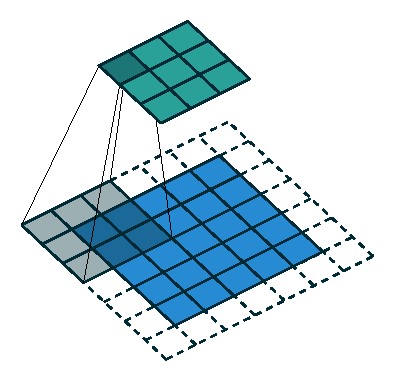
\includegraphics[width=0.24\textwidth]{images/padding_strides_00.pdf}
    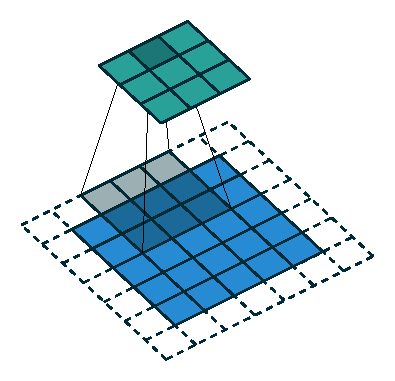
\includegraphics[width=0.24\textwidth]{images/padding_strides_01.pdf}
    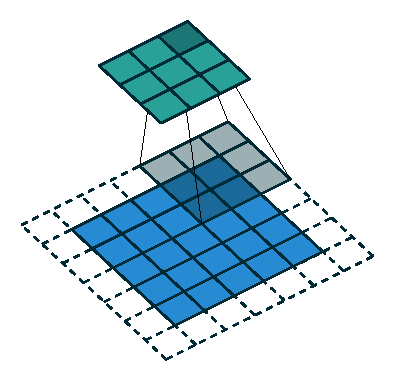
\includegraphics[width=0.24\textwidth]{images/padding_strides_02.pdf}
    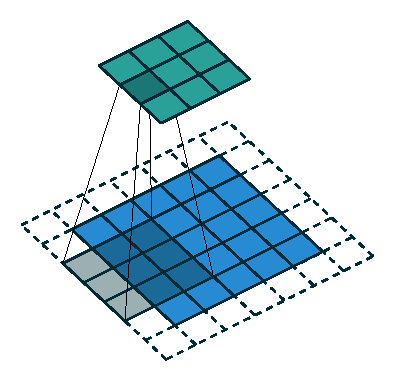
\includegraphics[width=0.24\textwidth]{images/padding_strides_03.pdf}
    \caption[2D convolution with padding and strides]{\label{fig:convolution_padding_strides}Convolving a 3×3 kernel over a 5×5 input padded with
    a 1×1 border of zeros using 2×2 strides. \cite{convolutionguide}}
\end{figure}

Convolution can also be represented as a multiplication of the input by matrix $\mathbf C $. An example of such matrix for the same case as in figure \ref{fig:convolution_slide}  can be seen in figure \ref{fig:convolution_matrix}.

\begin{figure}[ht]
    \centering
    \resizebox{0.95\hsize}{!}{$\begin{pmatrix}
        w_{0,0} & w_{0,1} & w_{0,2} & 0       & w_{1,0} & w_{1,1} & w_{1,2} & 0       & w_{2,0} & w_{2,1}   & w_{2,2}   & 0       & 0       & 0       & 0       & 0       \\
        0       & w_{0,0} & w_{0,1} & w_{0,2} & 0       & w_{1,0} & w_{1,1} & w_{1,2} & 0       & w_{2,0}   & w_{2,1}   & w_{2,2} & 0       & 0       & 0       & 0       \\
        0       & 0       & 0       & 0       & w_{0,0} & w_{0,1} & w_{0,2} & 0       & w_{1,0} & w_{1,1}   & w_{1,2}   & 0       & w_{2,0} & w_{2,1} & w_{2,2} & 0       \\
        0       & 0       & 0       & 0       & 0       & w_{0,0} & w_{0,1} & w_{0,2} & 0       & w_{1,0}   & w_{1,1}   & w_{1,2} & 0       & w_{2,0} & w_{2,1} & w_{2,2} \\
    \end{pmatrix}$}
    \caption[Convolution represented as matrix multiplication]{\label{fig:convolution_matrix}Convolution with 4×4 input and 3×3 kernel represented as matrix multiplication. Inputs and outputs are concatenated. }
\end{figure}

We can see that multiplying the input by this matrix gives us the same result as sliding the kernel window over the input. The backward pass is easily obtained from this representation by transposing $\mathbf C$. The error is backpropagated by multiplying the loss with $\mathbf C^T$.

If we look at the matrix, we can see the properties of convolution mentioned above. This representation is closer to the actual implementation used in \glspl{NN}, as it employs matrix multiplication \footnote{Software implementations will typically not perform the useless zero multiplications.}. The matrix is sparse. Therefore fewer parameters need to be stored, reducing memory requirements. It also means we can compute the convolution result faster than in the fully connected case. These efficiency improvements are pretty significant. Most algorithms used in practice run in $O(mn)$ time where $m$ and $n$ are input and output sizes, respectively. For kernel with $k$ parameters, convolution can be run in $O(kn)$ time. Speed improvement is evident when we realize that $k$ can often be orders of magnitude smaller than $m$ while obtaining a good performance.

Parameter sharing can also be seen in the matrix. Kernel weights are reused multiple times, unlike in traditional \gls{NN}, where each element of the weight matrix is used only once. Parameter sharing does not affect the forward propagation's runtime but further reduces the model's storage requirements.

Equvariance to translation is another property of \glspl{CNN}. Equivarience of function $f(x)$ to function $g$ means that $f\left(g(x)\right) = g\left(f\left(x\right)\right)$. In other words, equivariance to translation means that if I shifted the input by some number of pixels, I would get the same output but also shifted by the same amount. It is perhaps harder to see from the examples, but it is nonetheless useful. \cite[pg. 329-335]{deeplearningbook}

\gls{CNN} is defined as a \gls{NN} that has at least one convolutional layer.

\subsection{Transposed Convolution}
\label{subsec:transposed_convolution}

Transposed convolutions are quite useful, especially in generative models. The need arises from the desire to use a transformation that goes in the opposite direction of normal convolution. It is easy to assume that transposed convolution is the ``opposite'' operation of a regular convolution without giving it much thought. Its purpose is to go from something with the shape of some convolution output to something with the shape of its input. This operation should be done while maintaining a consistent connectivity pattern with said convolution. It is important to remember that there does not exist a reverse operation for convolution\footnote{Sometimes the term ``deconvolution'' is used instead of transposed convolution, which may be misleading.}. \cite{convolutionguide, deconvolutionbias}

Every convolution boils down to an efficient implementation of a matrix operation. A transposed convolution works by swapping forward and backward passes of a convolution. One kernel defines matrix $\mathbf C$, an example of which can be seen in figure \ref{fig:convolution_matrix}, and its transposition $\mathbf C^T$. The matrix used for a forward and backward pass determines the convolution type. In the transposed convolution, $\mathbf C^T$ is used for the forward pass instead of $\mathbf C$ in standard convolution.

It is always possible to emulate a transposed convolution with a direct convolution. The disadvantage is that it usually involves adding many columns and rows of zeros to the input, resulting in a much less efficient implementation. It is a more useful representation of transposed convolution. It is necessary to zero-pad the input if the same connectivity pattern, in the equivalent convolution to the transposed one, is to be maintained. It must be done so that the kernel's first (top-left) application only touches the top-left pixel.

Suppose we now imagine a convolution with non-unit strides and an ``opposite'' transposed convolution to it. In that case, the strides in the transposed convolution need to be fractional, as we are now increasing the output's size. Hence, we need to take steps smaller than one\footnote{This is why transposed convolution is sometimes also called fractionally-strided convolution.}. Fractional steps can be achieved in the representation of transposed convolution by the standard one by inserting zeros between input units. Inserting zeros between rows and columns of the input makes the kernel move around at a ``slower pace'' than with unit strides\footnote{The padding has to be equal to the size of the kernel minus one.}. Figure \ref{fig:convolution_padding_strides_transposed} illustrates the fractional strides. Transposed convolution in figure \ref{fig:convolution_padding_strides_transposed} is ``opposite'' of the convolution in figure \ref{fig:convolution_padding_strides}. \cite{convolutionguide}
\footnote{For more visualizations and a deeper explanation of how different convolution parameters, such as padding and strides, influence the output size, you can refer to \cite{convolutionguide}.}

\begin{figure}[ht]
    \centering
    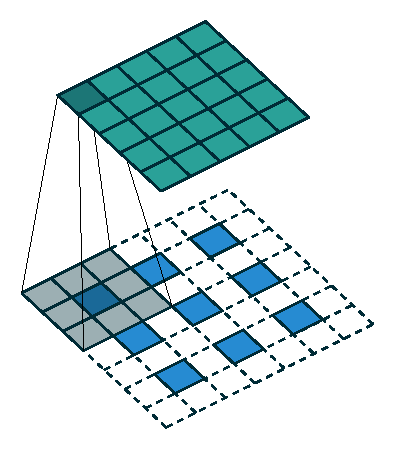
\includegraphics[width=0.24\textwidth]{images/padding_strides_transposed_00.pdf}
    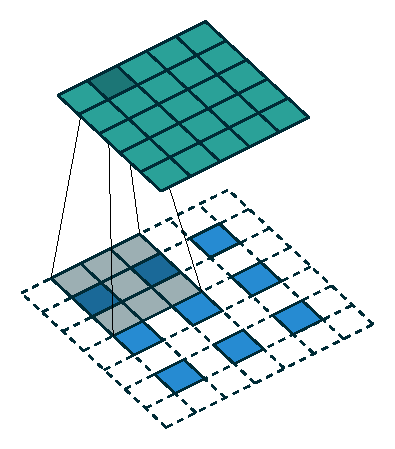
\includegraphics[width=0.24\textwidth]{images/padding_strides_transposed_01.pdf}
    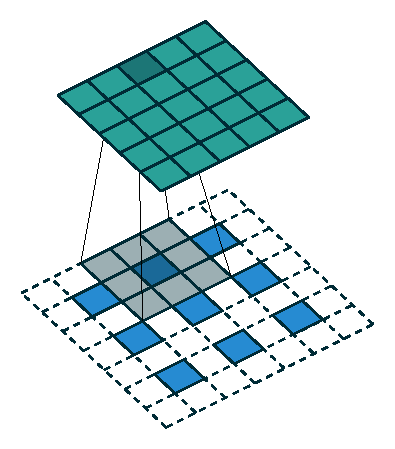
\includegraphics[width=0.24\textwidth]{images/padding_strides_transposed_02.pdf}
    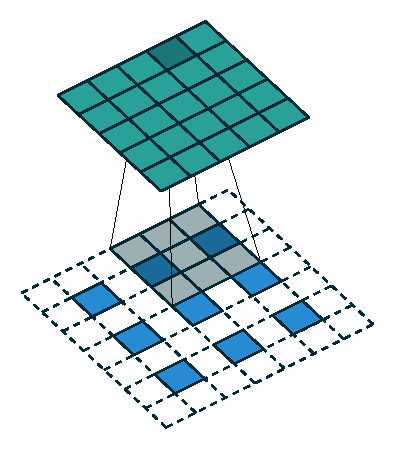
\includegraphics[width=0.24\textwidth]{images/padding_strides_transposed_03.pdf}
    \caption[2D transposed convolution]{\label{fig:convolution_padding_strides_transposed}
    Transposed convolution to convolving a 3×3 kernel over a 5×5 input padded with a 1×1 border of zeros using 2×2 strides (figure \ref{fig:convolution_padding_strides}). It is equivalent to convolving a 3×3 kernel over a 3×3 input (with
    one zero inserted between inputs) padded with a 1×1 border of zeros using unit
    strides. \cite{convolutionguide}}
\end{figure}

\subsection{Pooling}
\label{subsec:pooling}

Pooling operations reduce the size of the feature maps by using some function to summarize subregions of the input, such as taking the average or the maximum value. Pooling works like discrete convolution as it slides a window across the input, but it uses a different function instead of the linear combination used in convolution. In addition to discrete convolutions, the pooling operation makes up another vital building block in \glspl{CNN}.

\subsection{Validation Metrics}
\label{subsec:val_metrics}

Different evaluation metrics are used for assessing the performance of \glspl{CNN}, particularly in image processing and computer vision tasks. Here is a brief overview of metrics that I will use later in the thesis.
\begin{itemize}
    \item \gls{SSIM} is a perceptual metric that quantifies the similarity between two images. It considers the images' luminance, structure information, and contrast, which are more aligned with human visual perception. \gls{SSIM} values range from -1 to 1, with 1 indicating a perfect match between the two images. In the context of \glspl{NN}, \gls{SSIM} can be used to evaluate the quality of generated or reconstructed images, such as in image denoising, super-resolution, or image-to-image translation tasks.
    \item \gls{MAE} is a simple and easy-to-interpret metric that measures the average absolute difference between the predicted and actual values. It is used for both regression and image-processing tasks. For image processing, \gls{MAE} calculates the average absolute difference between the pixel values of two images. A lower \gls{MAE} indicates better model performance, which signifies fewer predicted and actual value discrepancies.
    \item \gls{MSE} is another metric used to measure the difference between predicted and actual values. It calculates the average squared difference between the two sets of values. In image processing, \gls{MSE} measures the average squared difference between the pixel values of two images. Similar to \gls{MAE}, a lower \gls{MSE} value indicates better performance. \gls{MSE} tends to penalize more significant errors more severely than MAE, as the squared term magnifies the differences.
\end{itemize}

Figure \ref{fig:metric} captures differences between each metric. These metrics are used to evaluate and compare the performance of different neural network models or configurations in various tasks, such as image synthesis, denoising, segmentation, and more. Models can be fine-tuned to achieve better results by analyzing the performance using these metrics.

\begin{figure}[ht]
    \centering
    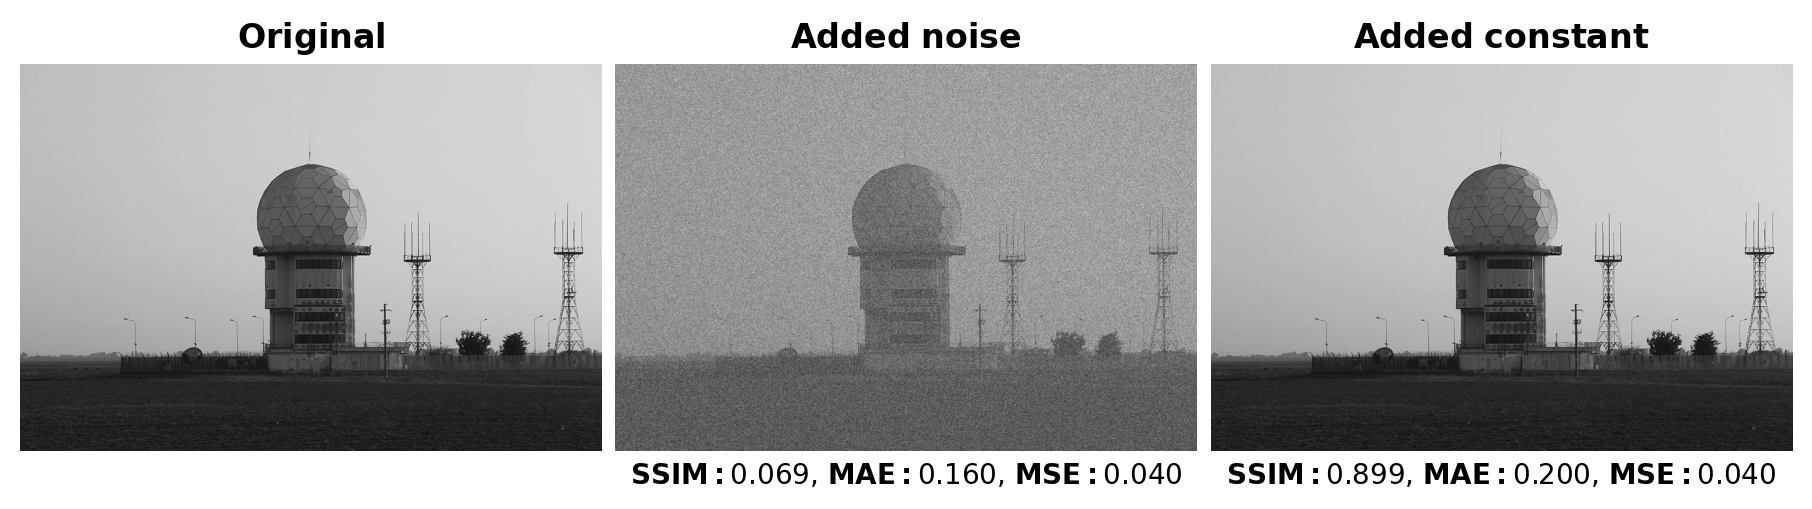
\includegraphics[width=\textwidth]{images/metrics.png}
    \caption[Differences between evaluation metrics]{\label{fig:metric}Differences between evaluation metrics. Modified images have the same \gls{MSE}, but one was created from the original by adding a random noise and the other by adding a constant. Image used for the comparison: \cite{wiki}.}
\end{figure}

\section{UNet}
\label{sec:unet}

UNet is a \gls{CNN} that was first proposed for biomedical image segmentation in the paper \cite{unet}. The architecture of this network consists of there main parts, encoder layers, bottleneck, and decoder layers. Encoders are typical convolution layers that consist of convolution stage, nonlinearity, and pooling stage\footnote{There are two conventions when it comes to the term ``layer'' in \glspl{CNN}. In one, the convolution, nonlinearity, and pooling are all called layers, and in the other layer is a term for all of them together. I will use the latter one.}. The convolution and nonlinearity stages can be repeated multiple times in one layer. A diagram showing this layer can be seen in figure \ref{fig:unet_encoder_layer}. The pooling stage reduces the resolution of the images. The convolution inside the encoder is also used for increasing the number of features.

\begin{figure}[ht]
    \centering
    \begin{subcaptionblock}[c]{\textwidth}
        \centering
        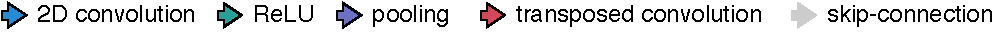
\includegraphics[width=\textwidth]{images/unet_legend.pdf}
    \end{subcaptionblock}
    \begin{subcaptionblock}[t]{.45\textwidth}
        \centering
        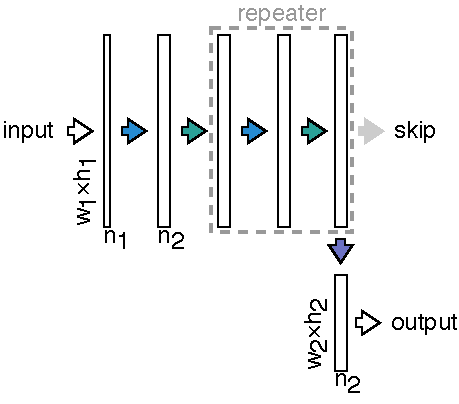
\includegraphics[height=0.8\textwidth]{images/unet_encoder.pdf}
        \caption[One layer of UNet decoder]{\label{fig:unet_encoder_layer}Encoder}
    \end{subcaptionblock}
    \begin{subcaptionblock}[t]{.45\textwidth}
        \centering
        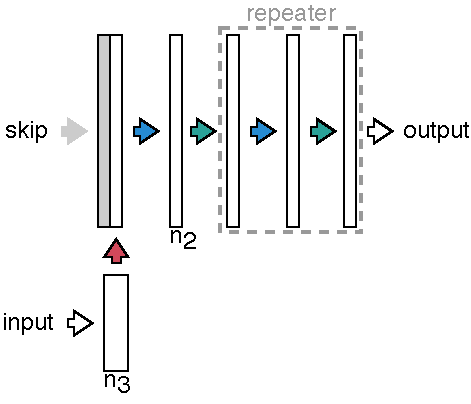
\includegraphics[height=0.8
        \textwidth]{images/unet_decoder.pdf}
        \caption[One layer of UNet decoder]{\label{fig:unet_decoder_layer}Decoder}
    \end{subcaptionblock}
    \caption[Types of layers in the UNet architecture]{\label{fig:unet_layers}Types of layers in the UNet architecture}
\end{figure}


Figure \ref{fig:unet_decoder_layer} illustrates that the decoder layer starts with upsampling the output of the previous decoder layer or bottleneck. Upsampling is done using a transposed convolution, which increases the resolution and decreases the number of features. The bottleneck is practically the same as the encoder layer but without the pooling stage at the end.

Each encoder layer in the architecture acts as a low-pass filter, suppressing details and higher spatial frequencies in the input. For the higher frequencies to be transmitted to the output, the encoder must acquire the ability to encode them in the intermediate features of the network. \cite{gunet}

The original paper \cite{unet} introduced skip-connections in order to achieve this goal. These concatenate the encoder features before the pooling stage with the upsampled features in the decoder. Concatenation is done at each ``level'' of the network, effectively bypassing the network's lower levels. These ``fast-forward'' connections, as they are sometimes called, allow for the details from the input to be transferred directly to the output without passing them through a bottleneck. Removing the need to encode the higher spatial frequencies allows, the lower levels to better capture global features. Skip connections can be seen in figures \ref{fig:unet_layers} and \ref{fig:unet_architecture}.

Similarly to the encoder, convolution with activation stages can be repeated multiple times in the decoder.

\begin{figure}[ht]
    \centering
    \begin{subcaptionblock}{\textwidth}
        \centering
        \begin{tikzpicture}[scale=.35,every node/.style={minimum size=1cm}, on grid]
            \draw[thick, fill=blue] (0,0) rectangle (1,-4);
            \draw[thick] (0.5,-4.5) to (0.5,-6);
            \draw[->, thick]  (0.5, -6) to (1.5, -6);
            \draw[thick, fill=blue] (2,-5) rectangle (4,-7);
            \draw[thick] (3,-7.5) to (3,-8.5);
            \draw[->, thick]  (3, -8.5) to (4.5, -8.5);
            \draw[thick, fill=violet] (5,-8) rectangle (9,-9);
            \draw[thick]  (9.5, -8.5) to (11, -8.5);
            \draw[->,thick] (11,-8.5) to (11,-7.5);
            \draw[thick, fill=cyan] (10,-5) rectangle (12,-7);
            \draw[thick]  (12.5, -6) to (13.5, -6);
            \draw[->,thick] (13.5,-6) to (13.5,-4.5);
            \draw[thick, fill=cyan] (13,0) rectangle (14,-4);

            \draw[->,thick,draw=gray, dashed] (1.5,-2) to (12.5,-2);
            \draw[->,thick,draw=gray, dashed] (4.5,-6) to (9.5,-6);
        \end{tikzpicture}
    \end{subcaptionblock}
    \begin{tikzpicture}[scale=0.2,every node/.style={minimum size=1cm}, on grid]
        \begin{scope}[xshift=0cm,yshift=0cm]
            \draw[draw=base03,fill=blue,thick](0,0) rectangle (1, 1);
            \node[thick,anchor=west, text centered] (p3) at (1, 0.5) {Encoder};
        \end{scope}
        \begin{scope}[xshift=12cm,yshift=0cm]
            \draw[draw=base03,fill=violet,thick](0,0) rectangle (1, 1);
            \node[thick,anchor=west, text centered] (p3) at (1, 0.5) {Bottleneck};
        \end{scope}
        \begin{scope}[xshift=24cm,yshift=0cm]
            \draw[draw=base03,fill=cyan,thick](0,0) rectangle (1, 1);
            \node[thick,anchor=west, text centered] (p3) at (1, 0.5) {Decoder};
        \end{scope}
    \end{tikzpicture}

    \caption[UNet architecture]{\label{fig:unet_architecture}UNet architecture}
\end{figure}

The architecture can be designed for tiling to take advantage of the properties of \glspl{NN} that I mentioned, particularly the equivariance to translation. Tiling means that the \gls{NN} output can be extended without increasing the network size by running the net on different ``tiles'' of the image separately to produce output in a mosaic. For this to work near the edges of the tiles, the convolutional stages cannot have padding, which means the output of the \gls{NN} will be smaller than the input. An example of this can be seen in paper \cite[fig. 2]{unet}.

\section{Bias in Neural Networkts}
\label{sec:bias}

Bias in machine learning, also sometimes called algorithm bias or AI bias, is a phenomenon that occurs when an algorithm produces systemically prejudiced results. It is separate from the bias parameter inside \glspl{NN}.

\subsection{Structural Bias}
\label{subsec:structural_bias}

\begin{figure}[ht]
    \centering
    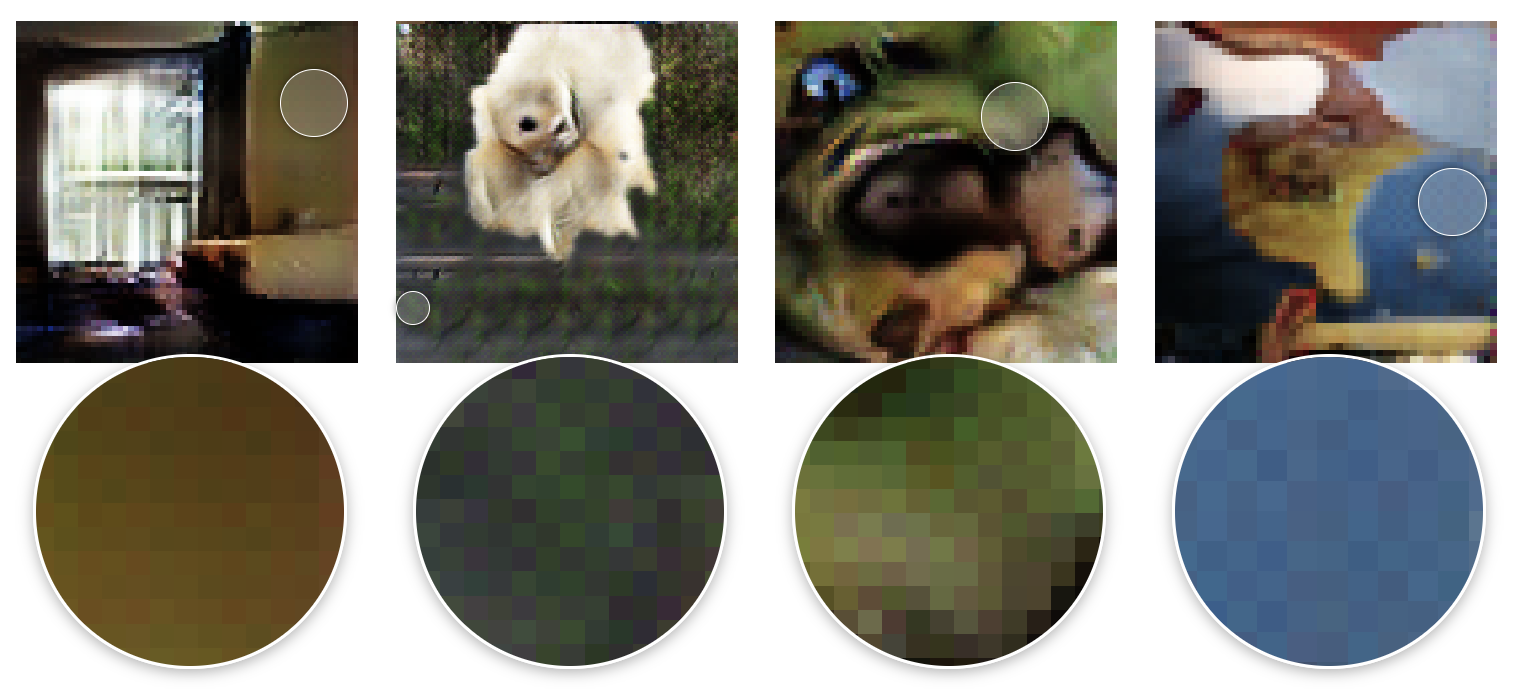
\includegraphics[width=\textwidth]{images/checkerboard_artefacts_models.png}
    \caption[Grid patterns in generative models]{\label{fig:grid_patterns_in_models}These instances show generative models that exhibit checkerboard artifacts in their outputs. The image used is sourced from \cite{deconvolutionbias}.}
\end{figure}


Many \gls{CNN} architectures employed a similar architecture to the one described in the section \ref{sec:unet} about UNet. When examining images created by these \glspl{CNN}, one may observe a distinct checkerboard pattern of irregularities, as shown in figure \ref{fig:grid_patterns_in_models}. When generating images from \glspl{NN}, the common practice is to start from lower-resolution images and gradually upscale them, which allows the \glspl{NN} to describe the rough image and then fill in some details in multiple steps. In order to achieve this, a technique for converting low-resolution images into high-resolution images is required. Transposed convolution is a commonly used method for this task, as explained in section \ref{subsec:transposed_convolution}. Layers of transposed convolutions are often found in the decoder of AutoEncoders or the generator part of \glspl{GAN}. The UNet is based on the AutoEncoder architecture and therefore uses transposed convolution.

Unfortunately, transposed convolution can easily lead to artifacts due to uneven overlap. In particular, uneven overlap in transposed convolution happens, when the kernel size is not divisible by the stride. In the section \ref{subsec:transposed_convolution}, I talked about fractional strides in transposed convolution and how they can be pictured as padding between input columns and rows. It is evident from the visualization in figure \ref{fig:transposed_convolution_artefacts} that the kernel occasionally overlaps one, two, or four inputs. This behavior forms grid-like artifacts. \glspl{CNN} generally have multiple layers with transposed convolution, so these artifacts compound on each other. \cite{deconvolutionbias}

\begin{figure}[ht]
    \centering
    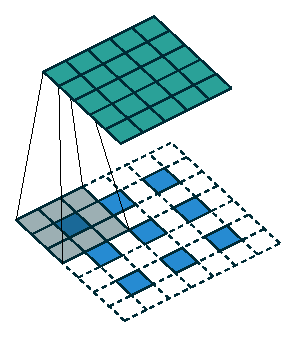
\includegraphics[width=0.24\textwidth]{images/transposed_artefacts_1.pdf}
    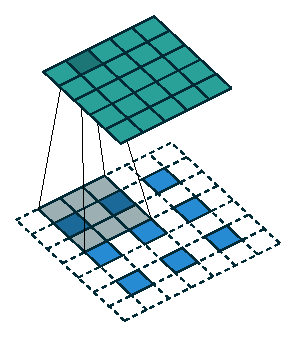
\includegraphics[width=0.24\textwidth]{images/transposed_artefacts_2.pdf}
    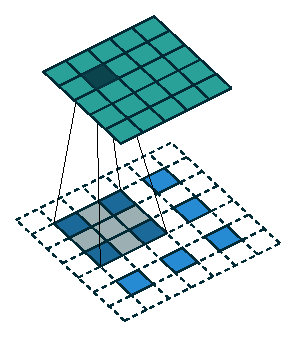
\includegraphics[width=0.24\textwidth]{images/transposed_artefacts_4.pdf}
    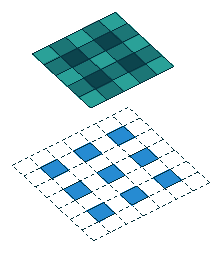
\includegraphics[width=0.24\textwidth]{images/transposed_artefacts_finished.pdf}
    \caption[Demonstration of artifact formation in transposed convolution ]{\label{fig:transposed_convolution_artefacts}
    Demonstration of artifact formation on the same transposed convolution as in figure \ref{fig:convolution_padding_strides_transposed}. \cite{convolutionguide}}
\end{figure}

The models are learning weights used in convolution and, in theory, could learn to mitigate the effects of uneven overlap. Learning to reduce these artifacts can be challenging, particularly when the convolution is done on multiple channels that impact each other. While possible, it significantly restricts the potential filters and therefore sacrifices the model's capacity. In practice, \glspl{CNN} struggle with completely avoiding these artifacts. In fact, not only do \glspl{NN} with uneven overlap not learn to avoid this, but models with even overlap often learn kernels that cause similar artifacts! While it is not their default behavior the way it is for uneven overlap, it is still very easy for transposed convolution with even overlap to cause artefacts\footnote{Even overlap happens when the kernel size is divisible by the stride.}. Completely avoiding artifacts in models with even overlap is still a significant restriction on filters, and in practice, the artifacts are still present in these models, although they seem milder.\cite{deconvolutionbias}

While many factors are at play here, the transposed convolution is a big part of the problem. It is fragile because it easily represents artifact-creating functions, even when the size is carefully chosen. At worst, creating artifacts is the default behavior of transposed convolution. In the upcoming section \ref{sec:guided_upsampling}, I will explain a method to increase the resolution of an image less susceptible to these visual abnormalities.

\subsection{Spectral Bias}
\label{subsec:spectral_bias}

Recent study \cite{spectralbias} focused on deep ReLU networks through the lens of Fourier analysis found that while \glspl{NN} can approximate arbitrary functions\footnote{See paper \cite{universalapproximators}}, they favor low-frequency ones. Therefore they exhibit a bias towards smooth functions. This phenomenon is called spectral bias. I will focus on two experiments in the study mentioned above.

In the first experiment, the researchers trained six layers deep and 256 unit wide fully-connected ReLU network on an output defined by the mapping $\lambda: [0, 1] \to \mathbb{R}$ given by

\begin{equation} \label{eq:experiment_1}
    \lambda(z) = \sum_i A_i \sin(2\pi k_i z + \varphi_i),
\end{equation}

\noindent where $\kappa = (k_1, k_2, ...)$ are the frequencies with corresponding amplitudes $\alpha = (A_1, A_2, ...)$ and phases $\phi = (\varphi_1, \varphi_2, ...)$. Network was trained to regress $\lambda$ with $\kappa = (5, 10, ..., 45, 50)$ and $N=200$ input samples spaced equally over $[0, 1]$. The spectrum of the output was monitored as training progressed. In the first setting, equal amplitudes $A_i = 1$ were set for all frequencies, and in the second setting, the amplitude gradually increased from $A_1 = 0.1$ to $A_{10} = 1$. Figure \ref{fig:spectralbias_experiment_1} shows that lower frequencies are regressed first, regardless of their amplitudes. \cite{spectralbias}

\begin{figure}[ht]
    \centering
    \begin{subcaptionblock}[t]{.475\textwidth}
        \centering
        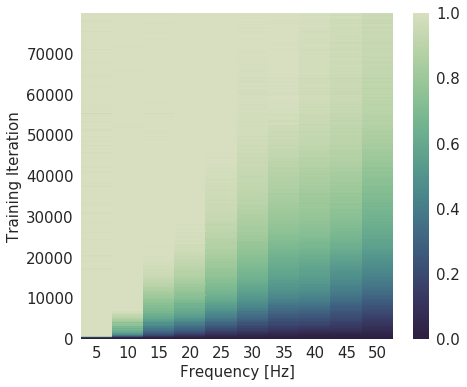
\includegraphics[height=0.9\textwidth]{images/experiment_1.png}
        \caption[Experiment showcasing spectralbias]{\label{fig:spectralbias_experiment_1}Evolution of the spectrum during training. The colors show the measured amplitude of the network spectrum at the corresponding frequency, normalized by the target amplitude at the same frequency. \cite{spectralbias}}
    \end{subcaptionblock}
    \hspace{1em}
    \begin{subcaptionblock}[t]{.475\textwidth}
        \centering
        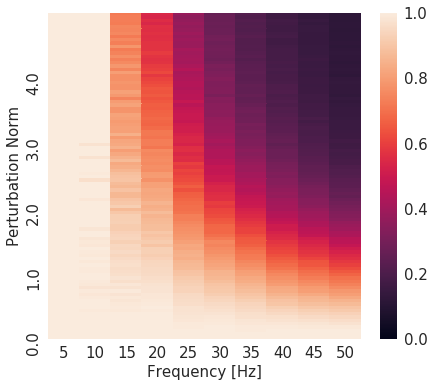
\includegraphics[height=0.9\textwidth]{images/experiment_2.png}
        \caption[Experiment showing robustness to parameter perturbation]{\label{fig:spectralbias_experiment_2}Spectrum of the model with perturbed parameters as a function of parameter perturbation. Amplitudes are normalized by the amplitudes obtained from the network without the perturbed parameters. \cite{spectralbias}}
    \end{subcaptionblock}
    \caption[Results of experiments showcasing the spectral bias]{\label{fig:spectralbias_experiments}Results of experiments from the study \cite{spectralbias} showcasing the spectral bias.}
\end{figure}

The same setup as the first experiment was used for the second experiment. Once the network had converged on certain parameters $\theta^{*}$, the authors made random perturbations $\theta = \theta^{*} + \delta \hat{\theta}$ of a specific size $\delta$, where $\hat{\theta}$ is a random unit vector in the parameter space. They evaluated the network function $f_{\theta}$ at the perturbed parameters and computed the magnitude of its discrete Fourier transform at frequencies $k_i$ to get $|\tilde{f}_{\theta}({k_i})|$. To obtain $|\tilde{f}_{\mathbb{E}\theta}({k_i})|$, which was then normalized by $|\tilde{f}_{\theta*}({k_i})|$, they averaged the results over 100 samples of $\hat{\theta}$. $|\tilde{f}_{\mathbb{E}\theta}({k_i})|$ was then averaged over the phases $\phi$ from equation \ref{eq:experiment_1},. Figure \ref{fig:spectralbias_experiment_2} displays the experiment's outcome. \cite{spectralbias}

The second experiment discovered that higher frequencies are more susceptible to changes in parameters than lower frequencies. This result suggests that precise tuning of the parameters is necessary for higher frequencies to be expressed effectively. In other words, parameters that contribute towards expressing high-frequency components occupy a small volume in the parameter space. \cite{spectralbias}

I hypothesize that the use of transposed convolution negatively impacts the learning of higher frequencies. It may not be possible to fine-tune the parameters required for capturing higher frequencies due to the limitations on filters in transposed convolution, as discussed in section \ref{subsec:transposed_convolution}. Increasing the likelihood of the model learning higher frequencies can be achieved by removing the structural biases that arise from upscaling using transposed convolution. In the following section \ref{sec:guided_upsampling}, I will focus on one upsampling method that aims to accomplish this by replacing the transposed convolution with guided upsampling.

\section{GUNet: Guided UNet}
\label{sec:guided_upsampling}

Transposed convolution in the decoder layers of the UNet architecture can cause checkerboard artifacts, as mentioned in section \ref{subsec:structural_bias}. Other non-learned upsampling methods can cause blurring since they are based on pre-defined interpolation.

Several methods that attempt to alleviate these upsampling artifacts have been proposed. A resize convolution technique is introduced in the research paper \cite{deconvolutionbias}. This method utilizes a technique that separates upsampling from convolution to ensure more precise feature computation. Before the convolution process, the image is resized using either nearest-neighbor or bilinear interpolation. Other methods try to reduce the checkerboard artifacts by correlating the kernel weights in transposed convolution. An example of such a method can be found in the paper \cite{aitken2017checkerboard}, which proposes a specialized initialization scheme for transposed convolutional layers that correlates the kernel weights at initialization. These methods generally eliminate the artifacts, but they fail to use the high-frequency details from the encoder efficiently and are trying to extract the information in the decoder. Non-learned methods are also prone to blurring. Furthermore, it should be noted that utilizing learned upsampling through transposed convolutions, even when the kernel weights are correlated, does not assure the avoidance of minima that produce artifacts during optimization, as previously discussed in section \ref{subsec:structural_bias}. \cite{gunet}

This section describes the \gls{GUNet} architecture proposed in the paper \cite{gunet}.

\subsection{Guided Image Filtering}
\label{subsec:guided_image_filtering}

\gls{GIF} is an edge-preserving smoothing filter. Its main advantage over bilateral filters is the computational complexity. The output image of the \gls{GIF} is consistent with the gradient direction of the guidance image, which prevents gradient reversal prominent in the bilateral filters.

\gls{GIF} works by assuming that there is a local linear model between the guidance $I$ and the filtering output $q$. The following definition of the filter is taken directly from the paper \cite{gif}, in which the filter was proposed.

\vspace{1em}
{\itshape
\noindent We assume that $q$ is a linear transform of $I$ in a window $\omega_{k}$ centered at the pixel $k$:

\begin{equation} \label{eq:linear_model}
    q_{i}=a_{k}I_{i}+b_{k}, \forall i \in \omega_{k},
\end{equation}

\noindent where $a_k$ and $b_k$ are some linear coefficients assumed to be constant in $\omega_{k}$. We use a square window of a radius $r$.

\noindent To determine the linear coefficients $a_k$ and $b_k$, we need constraints from the filtering input $p$. We model the output $q$ as the input $p$ subtracting some unwanted components $n$ like noise/textures:

\begin{equation}
    q_{i}=p_{i}-n_{i}.
\end{equation}

\noindent We seek a solution that minimizes the difference between $q$ and $p$ while maintaining the linear model in equation \ref{eq:linear_model}. Specifically, we minimize the following cost function in the window $\omega_{k}$:

\begin{equation} \label{eq:linear_ridge_regression}
    E(a_{k}, b_{k})=\sum_{i \in \omega_{k}}\big(\big(a_{k}I_{i}+b_{k}-p_{i}\big)^{2}+\epsilon a_{k}^{2}\big).
\end{equation}

\noindent Here, $\epsilon$ is a regularization parameter penalizing large $a_k$. Equation \ref{eq:linear_ridge_regression} is the linear ridge regression model, and its solution is given by

\begin{align} \label{eq:gif_coefficient}
    a_{k}={{1\over \vert \omega \vert } \sum_{i\in \omega_{k}}I_{i}p_{i}-\mu_{k}\bar{p}_{k}\over \sigma_{k}^{2}+\epsilon }, && b_{k}=\bar{p}_{k}-a_{k}\mu_{k}.
\end{align}

\noindent Here, $\mu_{k}$ and $\sigma_{k}^{2}$ are the mean and variance of $I$ in $\omega_{k}$, $\vert \omega \vert$ is the number of pixels in $\omega_{k}$, and $\bar{p}_{k} = \frac{1}{ \vert \omega \vert } \sum_{i\in \omega_{k}}p_{i}$ is the mean of $p$ in $\omega_{k}$. Having obtained the linear coefficients $a_k$ and $b_k$, we can compute the filtering output $q_i$ by equation \ref{eq:linear_model}.

\noindent However, a pixel $i$ is involved in all the overlapping windows $\omega_{k}$ that covers $i$, so the value of $q_i$ in equation \ref{eq:linear_model} is not identical when it is computed in different windows. A simple strategy is to average all the possible values of $q_i$. So after computing $a_k$ and $b_k$ for all windows $\omega_{k}$ in the image, we compute the filtering output by

\begin{equation} \label{eq:filtering_output}
    q_{i}={1\over \vert \omega \vert } \sum_{k \vert i \in \omega_{k}}(a_{k}I_{i}+b_{k}).
\end{equation}

\noindent Noticing that $\sum_{k \vert i \in \omega_{k}}a_{k}= \sum_{k \in \omega_{i}}a_{k}$ due to the symmetry of the box window, we rewrite equation \ref{eq:filtering_output} by

\begin{equation} \label{eq:gif}
    q_{i}=\bar{a}_{i}I_{i}+\bar{b}_{i},
\end{equation}

\noindent where $\bar{a}_{i} = {1\over \vert \omega \vert} \sum_{k \in \omega_i}a_k$ and $\bar{b}_{i} = {1\over \vert \omega \vert} \sum_{k \in \omega_i}b_k$ are the average coefficients of all windows overlapping $i$.

}
\vspace{1em}

The definition of the guided filter is provided by equations \ref{eq:gif_coefficient} and \ref{eq:gif}. Local linear model in equation \ref{eq:linear_model} ensures that $q$ has an edge only if $I$ has an edge because the gradient of $q$ is just scaled gradient of $I$ ($\nabla q=a \nabla I$). After the modifications in equation \ref{eq:gif}, this no longer holds true because the linear coefficients $\bar{a}_i$ and $\bar{b}_i$ vary spatially. Nevertheless, as $\bar{a}_i$ and $\bar{b}_i$ are the output of a mean filter, their gradients can be expected to be much smaller than that of $I$ near strong edges. In this situation, we can still have $\nabla q\approx \bar a \nabla I$, meaning that abrupt intensity changes in $I$ can be mostly preserved in $q$. \cite{gif}

The algorithm constructed from this definition runs in $O(N)$ and can be improved to $O(N/s^2)$, where $s$ is a subsampling ratio. Improve\-ment is achie\-ved using a \gls{FGF} described in paper \cite{fastguided}. In various applications, this leads to a speedup of more than ten times with almost no visible degradation. A pseudocode to both algorithms can be found in the appendix \ref{ax:gif}.

\subsection{Guided Upsampling}
\label{subsec:guided_upsampling}

Due to computational and memory costs, it is beneficial to downsample large images when performing image analysis and enhancement tasks such as tone mapping, colorization, stereo depth rendition, and photomontage. The result is then obtained by upsampling the solution computed on the smaller images. This upsampling does not consider the additional information in the original high-resolution image. Images upsampled by convolving the low-resolution image with an interpolation kernel typically also suffer from a blurring of sharp edges because of the smoothness inherent in the linear interpolation filters. A \gls{JBU} operation was proposed in the paper \cite{bilateral}, which leverages this information and produces outstanding full-resolution results from stereo depth rendition, image colorization, adaptive tone mapping, and graph-cut based image composition computed at very low resolutions.

Just like \gls{JBU}, \gls{GIF} can be utilized for upsampling by using an initial image as a basis for the operation. The algorithm differs from the one in section \ref{subsec:guided_image_filtering} because we now have a guidance image at a different scale than the filtering input. In this case, we compute the linear coefficient $a$ and $b$ in using the equation \ref{eq:gif_coefficient} at the coarse scale, bilinearly upsample them to the fine-scale (replacing the mean filter on $a$ and $b$) and compute the output by $q = aI + b$ at this scale. The result of \gls{GU} is visually comparable to the \gls{JBU}. \cite{gif}

\gls{GIF} provides a better performance than the bilateral filter used in \gls{JBU}, as I previously mentioned. The upsampling adjustments can also be made on \gls{FGF} for an even faster algorithm.

\subsection{Guided UNet Architecture}
\label{subsec:review_gunet_architecture}

\gls{GIF} can be incomported in the UNet architecture discussed in section \ref{sec:unet}. Using \gls{GIF}, we can benefit from the filter's edge-preserving nature and use the higher-level features from the encoder as guidance in the upsampling. UNet takes advantage of skip connections and combines them with features that pass through the bottleneck by concatenating them and combining them with convolution. \gls{GUNet} architecture proposed in paper \cite{gunet} replaces this with \gls{GU}.

In contrast to the UNet method, two skip connections are used in the upsampling process, which involves two levels of resolution: high and low. We can upscale the low-resolution feature by utilizing information from features in the skip connections of encoders from both levels.

Both of these features are used as guides in the filter. Let's call them $I^{\texttt{hr}}$ and $I^{\texttt{lr}}$. Input to the filter is an output of the previous decoder or bottleneck layer\footnote{When upsampling the bottleneck features in the first decoder, there is no skip-connection of lower-resolution we can use. One effective way to address this issue is to utilize the bottleneck as a lower resolution guide \textit{and} as an input for the filter.}. The illustrations of how this works can be found in figures \ref{fig:gunet_decoder} and \ref{fig:gunet_architecture}.

The operations of the \gls{GU} are modified to accommodate two guides. According to the paper \cite{gunet}, lower-resolution guide $I^{\texttt{lr}}$ and input $p$ are used to compute $\bar a_k^{\texttt{lr}}$ and $\bar b_k^{\texttt{lr}}$ on the lower resolution. The coefficients are then upsampled back to the higher resolution to form $\bar a_k^{\texttt{hr}}$ and $\bar b_k^{\texttt{hr}}$, using bilinear upsampling. The coefficients are then applied on the higher resolution guidance feature $I^{\texttt{hr}}$ to compute the final filtered decoder feature:

\begin{equation}\label{eq:guided_upsampling}
    q_i = \bar a_i^{\texttt{hr}}I^{\texttt{hr}} +\bar b_i^{\texttt{hr}}.
\end{equation}

The dotted arrows in figure \ref{fig:gunet_decoder} represent the abovementioned operations. Some readers might have noticed the discrepancy in the channel counts of lower coefficients ($\bar a_k^{\texttt{lr}}$, $\bar b_k^{\texttt{lr}}$) and higher coefficients ($\bar a_k^{\texttt{hr}}$, $\bar b_k^{\texttt{hr}}$). The authors of the paper state that the upsampling is done on each channel separately, but this poses a challenge, which I will discuss in the section \ref{subsed:channel_discrepancy}. One solution might be to use convolution to decrease channel counts of low-resolution coefficients.

\begin{figure}[h]
    \centering
    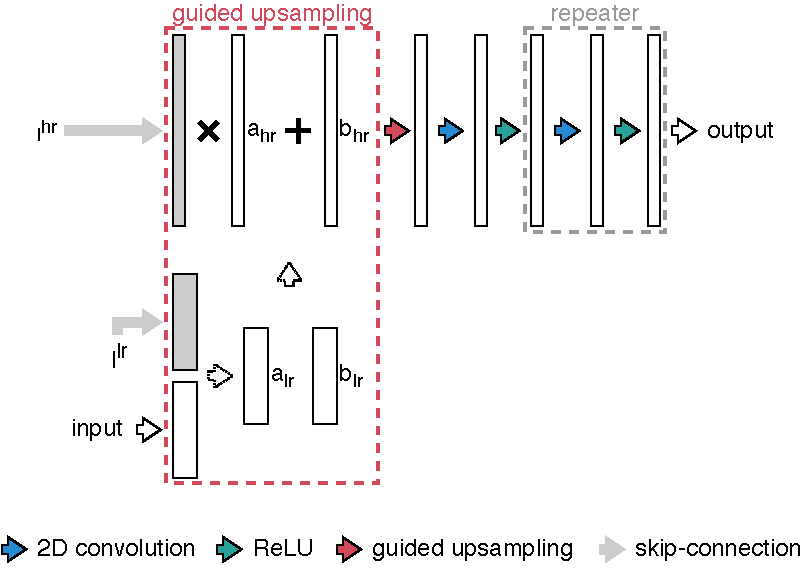
\includegraphics[width=0.8\textwidth]{images/gunet_decoder.pdf}
    \caption[Decoder layer in the GUNet architecture]{\label{fig:gunet_decoder}Decoder layer in the GUNet architecture}
\end{figure}

Guided feature upsampling combines the encoder and decoder features of the architecture and aims to guide its features at each upsampling stage in the output to be structurally similar to the corresponding feature set of the input features in the encoder. It is worth pointing out that \gls{GUNet} results in fewer parameters than UNets with transposed convolutions since the upsampling is parameter-free\footnote{Even if we use convolution to decrease the channel counts of the low-resolution coefficients $\bar a_k^{\texttt{lr}}$ and $\bar b_k^{\texttt{lr}}$} and the concatenation layer is avoided. The paper \cite{gunet} later investigates the effects of the structural biases of \glspl{CNN} on network outputs. The improvement attained by \gls{GUNet} was evident in the Fourier domain. The effectiveness of this approach was demonstrated in the inverse tone mapping and colorization of grayscale images. State-of-the-art performance was achieved in the inverse tone mapping application. In colorization, \gls{GUNet} exhibited benefits compared to alternative UNet architectures. \cite{gunet}

My goal is to apply this architecture to weather nowcasting and compare it with the traditional UNet both in the Fourier domain and using traditional metrics such as \gls{SSIM}, \gls{MAE}, and \gls{MSE}.

\begin{figure}[ht]
    \centering
    \begin{subcaptionblock}{\textwidth}
        \centering
        \begin{tikzpicture}[scale=.4,every node/.style={minimum size=1cm}, on grid]
            \draw[thick, fill=blue] (0,0) rectangle (1,-4);
            \draw[thick] (0.5,-4.5) to (0.5,-6);
            \draw[->, thick]  (0.5, -6) to (1.5, -6);
            \draw[thick, fill=blue] (2,-5) rectangle (4,-7);
            \draw[thick] (3,-7.5) to (3,-8.5);
            \draw[->, thick]  (3, -8.5) to (4.5, -8.5);
            \draw[thick, fill=violet] (5,-8) rectangle (9,-9);
            \draw[thick]  (9.5, -8.5) to (15, -8.5);
            \draw[->,thick] (15,-8.5) to (15,-7.5);
            \draw[thick, fill=cyan] (14,-5) rectangle (16,-7);
            \draw[thick]  (16.5, -6) to (17.5, -6);
            \draw[->,thick] (17.5,-6) to (17.5,-4.5);
            \draw[thick, fill=cyan] (17,0) rectangle (18,-4);

            \draw[->,thick,draw=gray, dashed] (1.5,-1.5) to (16.5,-1.5);
            \draw[->,thick,draw=gray, dashed] (5.5,-2.5) to (16.5,-2.5);
            \draw[thick,draw=gray, dashed] (5.5,-2.5) to (5.5,-5.5);

            \draw[->,thick,draw=gray, dashed] (4.5,-5.5) to (13.5,-5.5);
            \draw[->,thick,draw=gray, dashed] (10.5,-6.5) to (13.5,-6.5);
            \draw[thick,draw=gray, dashed] (10.5,-6.5) to (10.5,-8.5);
        \end{tikzpicture}
    \end{subcaptionblock}
    \begin{tikzpicture}[scale=0.2,every node/.style={minimum size=1cm}, on grid]
        \begin{scope}[xshift=0cm,yshift=0cm]
            \draw[draw=base03,fill=blue,thick](0,0) rectangle (1, 1);
            \node[thick,anchor=west, text centered] (p3) at (1, 0.5) {Encoder};
        \end{scope}
        \begin{scope}[xshift=12cm,yshift=0cm]
            \draw[draw=base03,fill=violet,thick](0,0) rectangle (1, 1);
            \node[thick,anchor=west, text centered] (p3) at (1, 0.5) {Bottleneck};
        \end{scope}
        \begin{scope}[xshift=24cm,yshift=0cm]
            \draw[draw=base03,fill=cyan,thick](0,0) rectangle (1, 1);
            \node[thick,anchor=west, text centered] (p3) at (1, 0.5) {Decoder};
        \end{scope}
    \end{tikzpicture}

    \caption[GUNet architecture]{\label{fig:gunet_architecture}GUNet architecture}
\end{figure}